% RecVis 2026, Assignment 3 report. CVPR 2024 author kit (cvpr.sty, ieeenat_fullname.bst).
\documentclass[10pt,twocolumn,letterpaper]{article}
\usepackage{cvpr}
\usepackage[dvipsnames]{xcolor}
\definecolor{cvprblue}{rgb}{0.21,0.49,0.74}
\usepackage[breaklinks,colorlinks,citecolor=cvprblue]{hyperref}

\def\paperID{A3}
\def\confName{RecVis}
\def\confYear{2026}

% Compact headings and title block: the report must fit on one page.
\makeatletter
\patchcmd{\@maketitle}{\vskip .5em}{}{}{\PackageError{report}{title patch 1 failed}{}}
\patchcmd{\@maketitle}{\vspace*{12pt}}{\vspace*{-2pt}}{}{\PackageError{report}{title patch 2 failed}{}}
\makeatother
\newcommand{\sect}[1]{\vspace{-2.2mm}\section{#1}\vspace{-2.4mm}}
\newcommand{\head}[1]{\par\vspace{0.5pt}\noindent\textbf{#1}}

\title{\vspace{-11mm}Learning from the Test Domain: 99.4\% Accuracy on Synthetic CIFAR-10\vspace{-3mm}}

\author{Elg\"un Hasanov \quad\textnormal{\large MVA RecVis 2026, Assignment 3 (Kaggle name: Elg\"un Hasanov)}\vspace{-11mm}}

\begin{document}
\maketitle

\sect{Introduction}
The training set is real CIFAR-10, but the 51,077 unlabelled test images are synthetic and stored at 32$\times$32 pixels.
A ResNet-18 trained on it reaches 85.4\% on validation and only 48.2\% on the public test set: the difficulty is the domain shift, not the ten classes.
My system therefore never trains on CIFAR-10.
It learns from the test domain itself in three stages (Tab.~\ref{tab:stages}) and reaches \textbf{99.41\%} public accuracy, first of 102 teams at the time of writing.

\sect{Method}
\noindent\textbf{Stage 1: zero-shot prior and graph (97.57\%).}
Two frozen models, PE-Core bigG/14~\cite{bolya2025pe} and SigLIP~2 g-opt/16~\cite{tschannen2025siglip2}, classify each upsampled image with the 80 ImageNet prompt templates~\cite{radford2021clip}; their probabilities are mixed 0.75/0.25, and the 6,241 least certain images get a flipped view.
Assuming that neighbours in feature space share a class, a $k$-NN graph over the test set ($k{=}20$, temperature 0.07) built on the features of both models and DINOv2 ViT-g/14~\cite{oquab2024dinov2} propagates the probabilities~\cite{zhou2003consistency}: \mbox{$p \leftarrow 0.5\,p_0 + 0.5\,Wp$}.

\head{Stage 2: self-training on the test set (98.05\%).}
I adapt the encoders to the test images: rank-8 LoRA adapters~\cite{hu2022lora} on every linear layer of each image tower are trained on soft targets (Stage~1 for bigG, the first bigG students for the other two).
Training is cross-fitted: a student trains on one half of the test set and predicts only the other, so it cannot confirm its own pseudo-labels.
The students then replace the frozen encoders.
I use three splits for bigG (one with strong augmentation~\cite{xie2020noisystudent}) and one for SigLIP~2 and DINOv2; a second bigG round on its own output was worse (97.60\%).

\head{Stage 3: labelled data from the test recipe (99.41\%).}
Two independent bigG students of Stage~2 disagree on only 0.7\% of the test images, so averaging more students could add little; I concluded that the remaining errors needed labels from the target domain.
The test images are the diffusion-hard part of CIFAR-10-W~\cite{sun2024cifar10w}; its paper names the generator, Stable Diffusion 2.1~\cite{rombach2022ldm}, and the 13 prompt templates.
I did not download or use any of its data.
I generated my own images with the public SD~2.1 weights (768px, 25 DPM-Solver steps, guidance 7.5) from these templates and the ten class names, so each image is labelled by its prompt.
Two label-free checks support this recipe: among the 20 nearest neighbours of a generated image in the Stage~1 feature space, 93.3\% are test images, against 94.2\% for held-out test images (SD~1.5: 81.8\%, SD-Turbo: 46.5\%); and of 18 ways to reduce to 32px, bicubic interpolation without antialiasing matches the radial power spectrum of the test images best.
A CLIP judge~\cite{fang2024dfn} removes the 0.5\% of images whose prompt class is not in its top two.
On the remaining 194,495 images I train DINOv2 ViT-g/14 with LoRA and a cosine classifier (3 epochs, label smoothing 0.1).
This student corrects Stage~2 only where it is uncertain: on the 8,664 test images below 0.9 confidence, both probability vectors are combined by a geometric mean.

\begin{table}[t]
\centering\small
\setlength{\tabcolsep}{4pt}
\begin{tabular}{@{}lr@{}}
\toprule
System & Public (\%) \\
\midrule
PE-Core bigG, zero-shot, 80 prompts & 96.65 \\
\quad + $k$-NN graph propagation & 97.00 \\
\quad + SigLIP 2 in prior and graph, selective flip & 97.36 \\
\quad + DINOv2-g features in the graph \hfill (Stage 1) & 97.57 \\
\quad + cross-fitted LoRA self-training \hfill (Stage 2) & 98.05 \\
\quad + DINOv2-g on 194k generated images \hfill (Stage 3) & \textbf{99.41} \\
\bottomrule
\end{tabular}
\vspace{-2mm}
\caption{Public accuracy after each step (rows are cumulative).}
\label{tab:stages}
\vspace{-3mm}
\end{table}

\begin{figure}[t]
\centering
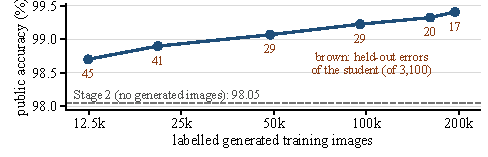
\includegraphics[width=\linewidth]{fig_scaling.pdf}
\vspace{-6mm}
\caption{Stage 3 with more data; each point is one trained student.}
\label{fig:scaling}
\vspace{-4mm}
\end{figure}

\sect{Results}
\noindent\textbf{Validation without test labels.}
I held out four ranges of generation seeds (18k images) and scored them with their prompt labels in the test graph: on 3,100 of them Stage~1 makes 82 errors and the final student alone 17.
More data helped at every size (Fig.~\ref{fig:scaling}; cf.~\cite{he2023synthetic}).
Beyond 50k images the held-out sets no longer separate consecutive students (3--5 errors apart on 4,940 images), so the public score became the more sensitive measure; between two files that differ in $m$ labels its noise is about $\sqrt{0.3m}/15{,}323$ (0.04--0.06 points here).
The last step gains about two such units; two- and four-seed ensembles (99.37\%) are within it.

\head{What did not help.}
Joint training with pseudo-labelled test images (98.83\% against 98.90\%), a supervised bigG student (57 against 45 held-out errors at four times the cost), and classifier heads fitted on images from other generators.

\head{Conclusion.}
Stages~1 and~2 added 1.4 points to the best single zero-shot model without any label, and labelled images generated with the test recipe added another 1.4.
My data is close to the test domain but not identical (unpublished sampler settings, cleaning by a model); the private score is not known yet.
All models have open weights; no test label was read, annotated or reconstructed.
CIFAR-10.1/10.2~\cite{recht2018cifar101,lu2020cifar102} and DomainNet~\cite{peng2019domainnet} served only to check early choices.

{\small
\bibliographystyle{ieeenat_fullname}
\bibliography{refs}
}
\end{document}
